\documentclass[11pt]{article}
\usepackage[margin=1in]{geometry}
\usepackage{graphicx}
\usepackage{booktabs}
\usepackage{float}

\title{ELEC5660 Project 1 Phase 2 Report}
\author{SIT, IOK LONG}
\date{\today}

\begin{document}
\maketitle

\section{Task}
I implemented three trajectory generators in the simulator:
Smooth Only, Minimum Jerk, and Minimum Snap.
All tests use Path 1.

\section{Method}
\begin{itemize}
\item Smooth Only: quintic piecewise polynomial, enforce position/velocity/acceleration continuity.
\item Minimum Jerk: equality-constrained QP, minimize integral of jerk squared.
\item Minimum Snap: equality-constrained QP, minimize integral of snap squared.
\end{itemize}

\section{Setup}
\begin{itemize}
\item Path: Path 1
\item Controller: default
\item Time allocation: equal segment time
\end{itemize}

\section{Results}

\begin{table}[H]
\centering
\begin{tabular}{lccc}
\toprule
Metric & Smooth & Min Jerk & Min Snap \\
\midrule
RMSE Position (m) & 0.1015 & 0.1011 & 0.1097 \\
RMSE Velocity (m/s) & 0.1477 & 0.1279 & 0.1397 \\
RMSE Yaw (deg) & 2.186 & 2.188 & 2.189 \\
Smoothness & 0.068 & 0.068 & 0.068 \\
\bottomrule
\end{tabular}
\caption{Path 1 comparison.}
\end{table}

\begin{figure}[H]
\centering
\begin{minipage}{0.32\linewidth}
\centering
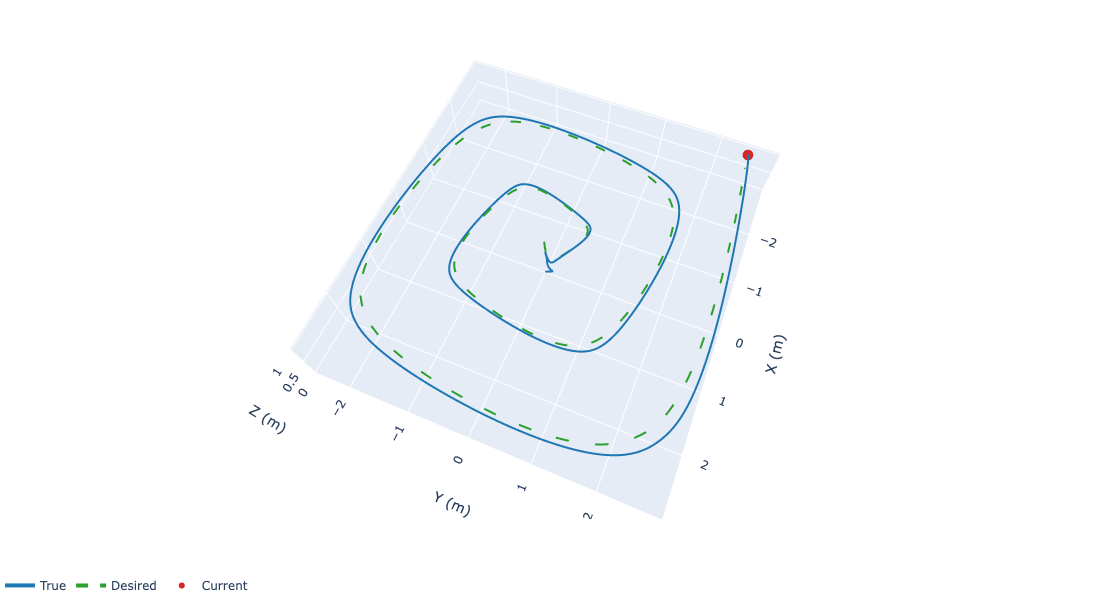
\includegraphics[width=\linewidth]{figs/smooth.png}
\caption*{Smooth}
\end{minipage}
\hfill
\begin{minipage}{0.32\linewidth}
\centering
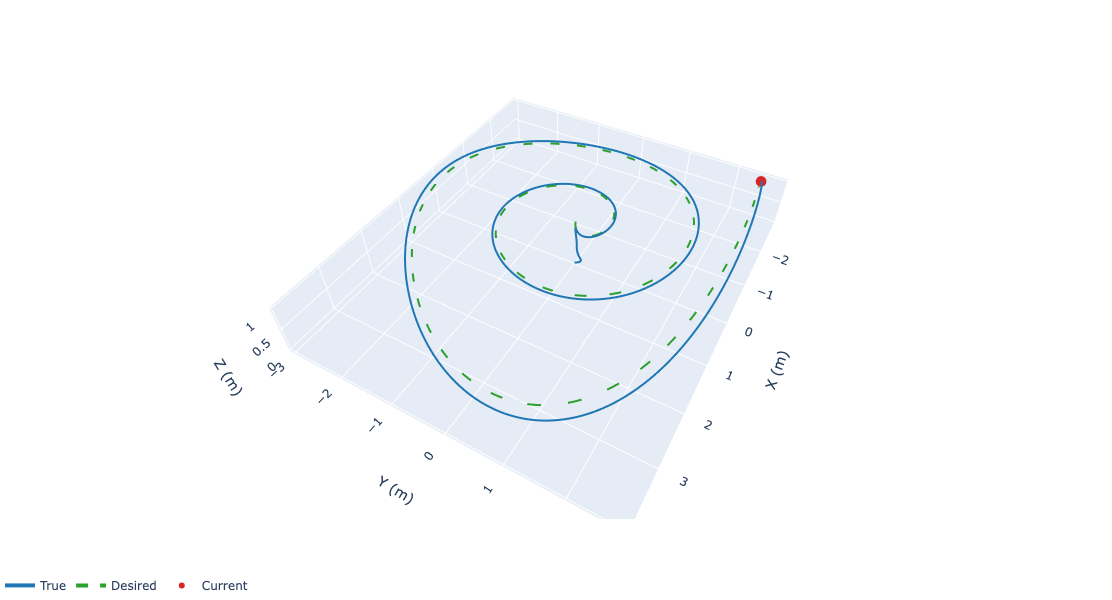
\includegraphics[width=\linewidth]{figs/jerk.png}
\caption*{Min Jerk}
\end{minipage}
\hfill
\begin{minipage}{0.32\linewidth}
\centering
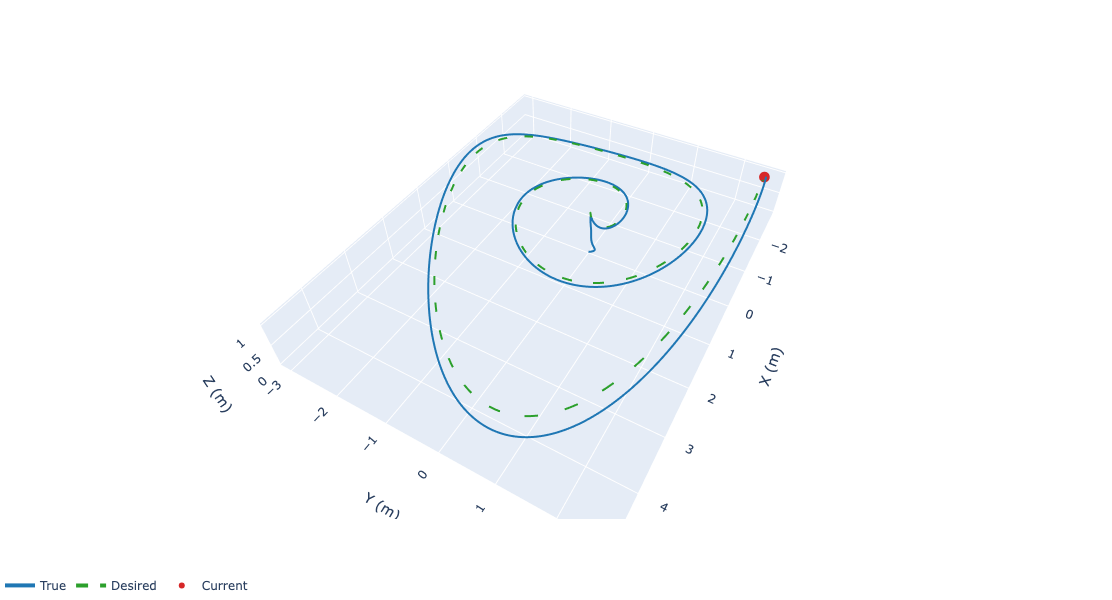
\includegraphics[width=\linewidth]{figs/snap.png}
\caption*{Min Snap}
\end{minipage}
\caption{Trajectory and tracking plots on Path 1.}
\end{figure}

\section{Discussion}
For Path 1, Min Jerk has the best RMSE position and RMSE velocity.
Min Snap is slightly worse than Min Jerk in this test.
Yaw RMSE and smoothness are almost the same for all three methods.

\section{Conclusion}
All three methods work and pass waypoints.
For this specific setup (Path 1), Minimum Jerk gives the best overall tracking result.

\section{References}
Course Lecture 4 slides and project starter code.

\end{document}